\section{Szótár generálása ismeretlen szavakból}

\begin{figure}[h!]
  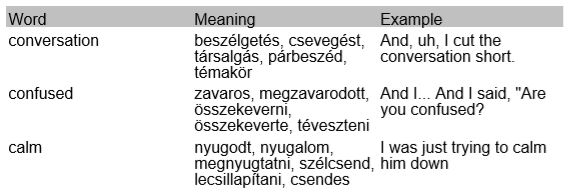
\includegraphics[width=\linewidth]{images/pdf.jpg}
  \caption{Ismeretlen szavakból generált szótár}
  \label{fig:pdf}
\end{figure}

Az alkalmazás képes fordítások megjelenítésére, valamint adatbázisba való elmentésükre, így a következő megvalósított funkció a szótárgenerálás volt. A szoftver az adatbázisból lekérdezés segítségével kinyeri a szükséges adatokat, majd ezekből egy \textit{.pdf} kiterjesztésű szószedetet állít elő. A \ref{fig:pdf}-es ábrán látható módon a szótár tartalmazza az ismeretlen szót, azaz a mondatelemet, amire a felhasználó kattintott, a jelentését vagy jelentéseit, valamint a kontextust, a mondatot, amelyben a kattintott elem szerepelt.

Először szükség volt egy függőség importálására az alkalmazás \textit{pom} fájljába. A választás az \textit{itextpdf} \textit{API}-jára esett, mely segítségével az említett funkcionalitás megvalósítása maradéktalanul kivitelezhető. Ezután a \textit{PDFGeneratorService} osztályt alkottam meg, amely a fájlgenerálásért felelős. Ebben található a \textit{createDictionary} metódus, amely az adatbázis adataiból a konkrét szószedetet kreálja. Egy új \textit{Document} objektum létrehozása után a \textit{PdfWriter} a dokumentum és egy \textit{FileOutputStream} segítségével hozza létre a merevlemezen a tényleges fájlt. A fájl neve alapesetben az aktuális feliratfájl nevével egyezik meg. Ezután egy táblázat kerül a dokumentumba, mely 3 oszlopból áll. A táblázat fejlécét az \textit{addTableHeader} függvény készíti el, így az tartalmazza a oszlopok feliratait, valamint egy világosszürke hátteret állít be neki. Az adatbázisból elkérjük az aktuális fájlnév alapján a rekordokat, majd ezen végig iterálunk, olyan módon, hogy minden rekordból egy \textit{Word} objektumot készítünk, amit pedig új sorként adunk a táblázathoz. A bejárás végeztével hozzáadjuk a táblázatot a dokumentumhoz, majd bezárjuk azt, ezzel lezárva a fájlt, és elérhetővé téve azt a felhasználónak. A folyamat forráskódját a \ref{lst:pdf}-as kódrészlet tartalmazza.

\begin{spacing}{1.25}
\begin{lstlisting}[caption=PDF fájl megalkotása, language=java, label={lst:pdf}]
document.open();
PdfPTable table = new PdfPTable(3);
addTableHeader(table);

for (Word word : new WordService()
.getAllByFilename(
PlayerControlsPanel.actualSubtitleFile.getName())) {
    addRow(table,
    word.getForeignWord(),
    word.getMeaning(),
    word.getExample());
}
document.add(table);
document.close();
\end{lstlisting}
\end{spacing}

E funkció megvalósításával lehetőség nyílt a felhasználó számára, hogy a neki ismeretlen szavakat és ezek jelentését kényelmesen hordozható formában elmentse. Ezáltal egy későbbi alkalommal, esetleg tanulás közben e szavak memorizálására fokozott figyelmet fordíthat, anélkül, hogy a kigyűjtésükhöz bármiféle plusz eszköz szükségeltetett volna, hiszen mindez filmnézés, szórakozás közben történt.